\documentclass{standalone}
\usepackage{tikz}
\usepackage{ctex,siunitx}
\setCJKmainfont{Noto Serif CJK SC}
\usepackage{tkz-euclide}
\usepackage{amsmath}
\usetikzlibrary{patterns, calc,3d}
\usetikzlibrary {decorations.pathmorphing,decorations.pathreplacing,decorations.shapes}
\tikzset{label style/.append style={font=\small}}
\begin{document}
\small
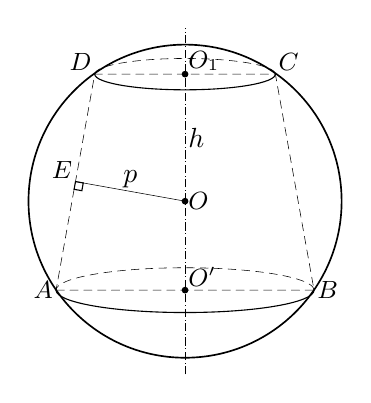
\begin{tikzpicture}[>=latex,scale=1.0,inner sep=1pt]
  \tkzDefPoints{0/0/O}
  \tkzDefPoint(1.1471,1.6134){C}
  \tkzDefPoint(-1.1471,1.6134){D}
  \tkzDefPoint(-1.6383,-1.1297){A}
  \tkzDefPoint(1.6383,-1.1297){B}
  \tkzDefMidPoint(C,D)\tkzGetPoint{O1}
  \tkzDefMidPoint(A,B)\tkzGetPoint{O'}
  % \draw[semithick](0,0)circle(2);
  \draw(C)arc(0:-180:{2*cos(55)} and {2*cos(55)*sin(10)});
  \draw[very thin,densely dashed](C)arc(0:180:{2*cos(55)} and {2*cos(55)*sin(10)});
  \draw(B)arc(0:-180:{2*cos(-35)} and {2*cos(-35)*sin(10)});
  \draw[very thin,densely dashed](B)arc(0:180:{2*cos(-35)} and {2*cos(-35)*sin(10)});
  \tkzDefPointsBy[projection=onto A--D](O){E}
  \tkzDrawPolygon[densely dashed](A,B,C,D)
  \tkzDrawSegments(O,E)
  \tkzDrawPoints[fill=black](O,O1,O')
  \tkzDrawCircle[semithick,black](O,A)
  \tkzLabelLine[pos=0.5,above](O,E){$p$}
  \tkzLabelLine[pos=0.5,right](O,O1){$h$}
  \tkzLabelPoints[left](A)
  \tkzLabelPoints[above left](D,E)
  \tkzLabelPoints[right](B,O)
  \tkzLabelPoint[above right](O1){$O_1$}
  \tkzLabelPoints[above right](C,O')
  \tkzMarkRightAngle[size=0.1](A,E,O)
  \draw[very thin,densely dashdotted](0,-2.2)--(0,2.2);
\end{tikzpicture}
\end{document}